\documentclass[11pt,a4paper]{emulateapj}

\usepackage{epsfig}
\usepackage{natbib}

\usepackage{ifpdf} \usepackage[bookmarks=false]{hyperref} \pdfoutput=1
\usepackage[usenames,dvipsnames]{color} \usepackage{graphicx}
\usepackage{graphics} \usepackage{float}
\usepackage{amsmath} \usepackage{amssymb} \usepackage{acronym}
\usepackage{comment} \usepackage{multirow} \usepackage{xspace}
\usepackage{units} \usepackage{dcolumn} \usepackage{ulem}

\def\aj{Astron. J.}  % Astronomical Journal 
\def\apj{Astrophys. J.}  %Astrophysical Journal 
\def\apjl{Astrophys. J. Lett.}  % Astrophysical Journal, Letters 
\def\pasj{PASJ} 
\def\apjs{Astrophys. J., Suppl. Ser.} % Astrophysical Journal, Supplement
\def\mnras{Mon. Not. R. Astron. Soc.}  % Monthly Notices of the RAS
\def\prd{Phys. Rev. D} % Physical Review D 
\def\prl{Phys. Rev. Lett.} % Physical Review Letters 
\def\cqg{Class. Quant. Grav.}%Classical and Quantum Gravity 
\def\araa{Annu. Rev. Astron. Astrophys.}  % Annual Review of Astron and Astrophys 
\def\nat{Nature} % Nature
\def\aap{Astron. Astrophys.}  % Astronomy and % Astrophysics
\def\jasa{J. Am. Stat. Assoc.}  
\def\pccp{Phys. Chem. Chem. Phys.}
\def\jrssb{J. R. Stat. Soc. B} 
\def\aipcs{AIP Conf. Ser.}
\def\jcp{J. Chem. Phys.}

\newcommand{\carl}[1]{{\color{red} #1}}

\begin{document}

\title{Title goes here} 
  \author{Carl L. Rodriguez\altaffilmark{1},}

\altaffiltext{1}{Center for Interdisciplinary Exploration and Research
  in Astrophysics (CIERA) \& Dept.~of Physics and Astronomy,
  Northwestern University, 2145 Sheridan Rd, Evanston, IL 60208, USA;
  [e-mail: {\tt cr@u.northwestern.edu}]}


\section{Comparison with N-Body}

The Monte Carlo approach requires one to compute the local average of several
physical quantities.  For instance, the physics of binary formation via
three-body encounters and the selection of the relaxation time both depend upon
local averages of the number density, velocity dispersion, and average mass of
the cluster at a specific radius \citep{2005MNRAS.358..572I,Joshi:2000tv}.
However, it is not the case that these averages should be computed over the same
number of stars.   While three-body binary formation should depend only on the
properties of the closest stars, the relaxation time step should be broadly
applied to the entire cluster.  We both expect and require three-body binary
formation to be more sensitive to local spikes in number density and velocity
dispersion than the cluster-wise relaxation time.  Therefore, we must adjust the
number of stars over which to compute an average depending on the scale of the
physics in question.

\begin{figure}[h!]
  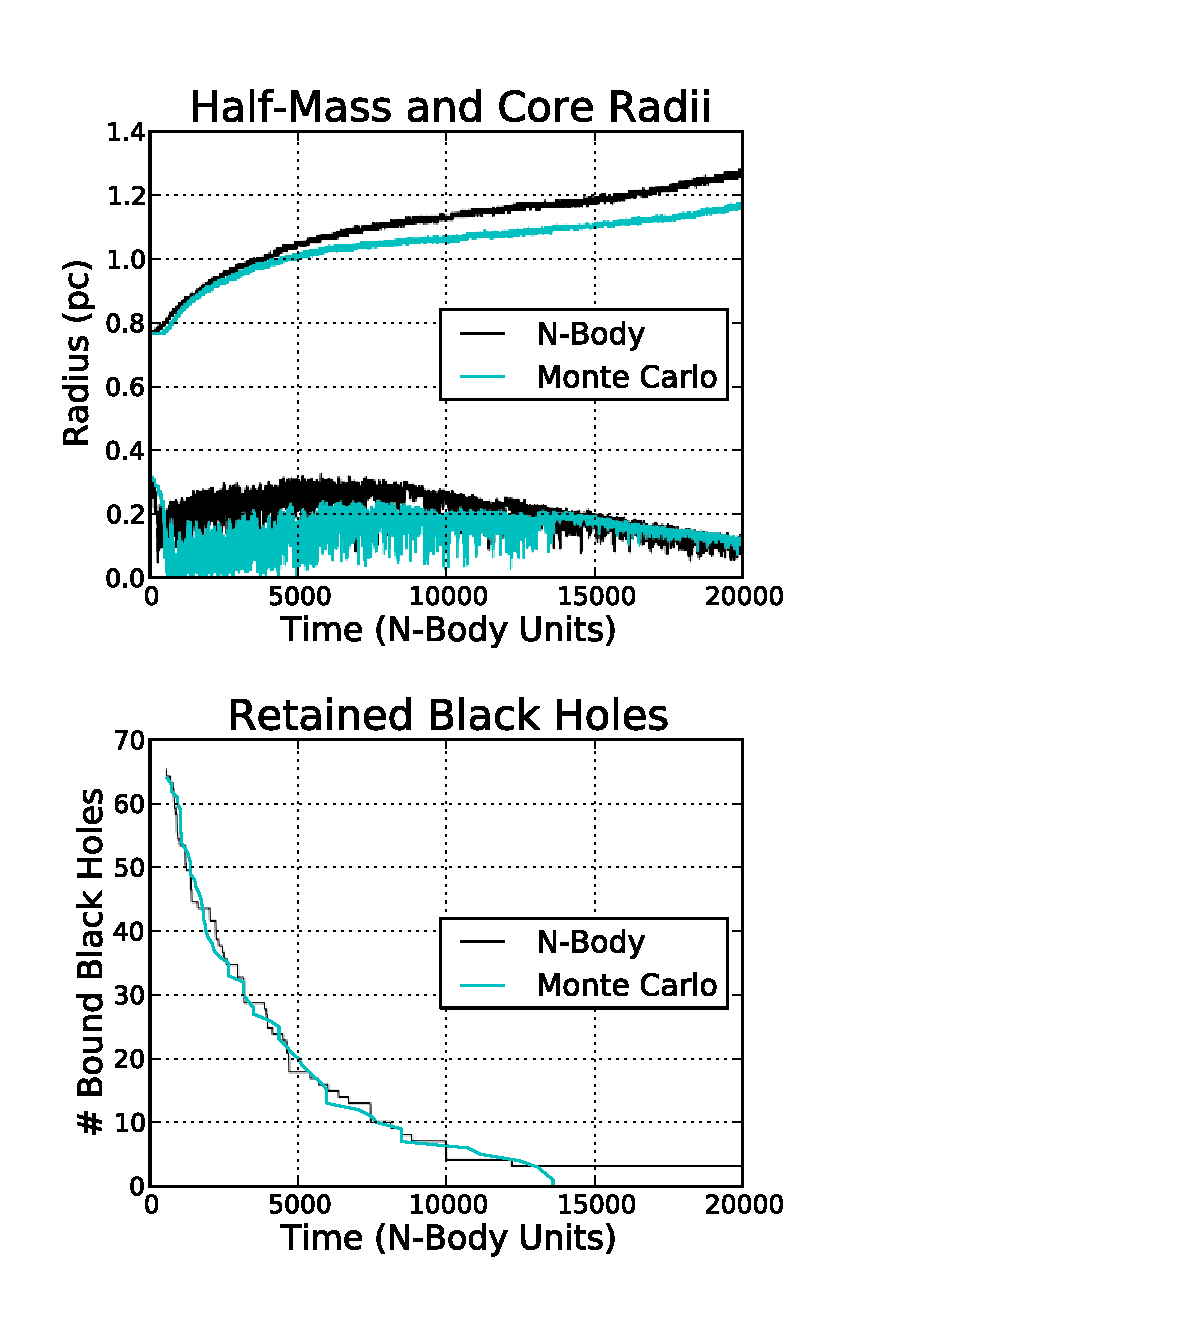
\includegraphics[scale=0.65]{64.pdf}
  \caption{Evolution of 2-Species Plummer models as computed by the Monte Carlo
  approach and the direct N-body approach of \cite{2013MNRAS.432.2779B}.  The
  top plot shows the half-mass radius (on top) and core radius (bottom) for the
  two methods, while the lower plot shows the number of retained black holes as
  a function of time.}
  \label{fig:2species64k}
\end{figure}


As in previous studies \citep{Joshi:2000tv} we determine the optimal code
parameters by direct comparison to N-body simulations with identical initial
conditions.  The primary focus of this study is the retention of black holes,
so we choose as our comparison an idealized two-component model recently studied 
in \cite{2013MNRAS.432.2779B}.  These models are a realization of standard Plummer
sphere populated by a large population of stellar mass objects and a smaller
population of heavy objects.  We consider models with an individual mass ratio of
$m_2/m_1 = 20$, and a total cluster mass ratio of $M_2/M_1 = 0.02$, where $m_1$
and $m_2$ are the masses of individual particles, and $M_1$ and $M_2$ are the
total masses of each component.  We consider runs with $64k$ and $128k$ number
of particles, although only the $64k$ runs are illustrated here.

In Fig. \ref{fig:2species64k}, we compare the cluster properties as reported by
the N-body simulations of \cite{2013MNRAS.432.2779B} to the results of our Monte
Carlo technique.  Empirically, we find optimal agreement by computing the
average quantities over the nearest 40 stars for two-body relaxation, and the
nearest 6 stars for three-body binary formation.  In particular, the 
evaporation rate of the black-hole subcluster from the Monte Carlo replicates
the N-body results extraordinarily well up to the ejection of the final
black-hole binary from the cluster.  Furthermore, we find the Monte Carlo
approach correctly replicates the half-mass expansion to within 8\% after
$2\times10^5$ N-body time units.  

Of the measured cluster properties, only the core radius cannot be
reproduced correctly by the Monte Carlo approach.  Immediately following core
collapse, the measured core radius for the Monte Carlo differs from the N-body
results by as much as 65\%.  Unfortunately this is to be expected: once mass
segregation and core collapse have occurred, the cluster core is comprised almost
entirely of black holes which have dynamically decoupled from the rest of the
cluster.  Correctly modelling the internal dynamics of an $N\sim100$ system using
a Monte Carlo has very little hope of success; however, as the black holes are
ejected, and the core becomes populated with a larger number of lighter halo
stars, the validity of the Monte Carlo approach is restored, and the core
radius better resembles that of the N-body approach.  New techniques are under
investigation that will correctly evolve the subcluster dynamics while
maintaining the speed of the Monte Carlo approach. 

\bibliographystyle{apj}
\bibliography{2speciesTuning.bib}{}
\end{document} 
